
\documentclass[10pt,xcolor=table]{beamer}
\usepackage[french]{babel}
\usepackage[T1]{fontenc}
\usepackage[utf8]{inputenc}
\usetheme{Warsaw}
\usepackage{pdfpages}


\begin{document}
%nico
\begin{frame}
  \frametitle{Introduction}

  \begin{itemize}[<+->]
  \item La Stéganographie,
  \item Origine de la cryptographie,
  \item Ronald Rivest et le cryptage RSA
  
  \begin{block}{Les 3 critères}
    \begin{itemize}
    \item Confidentialité,
    \item Authenticité,
    \item integrité
    \end{itemize}
  \end{block}
  \end{itemize}
  \pause
  \begin{center}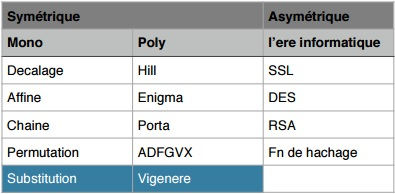
\includegraphics[scale=0.4]{Tab1.jpg}\end{center}

\end{frame}

\section{Développement}

\begin{frame}[<+->]
  \frametitle{Développement}
  
  \begin{exampleblock}{Produit sur le marché}
	\begin{enumerate}
    \item www.decode.fr,
    \item Decrypto (Google Play Store),
    \item Axcypte
    \end{enumerate}
  \end{exampleblock}

  \begin{block}{Phase de développement}
   
    \begin{enumerate}
    \item Identification,
    \item Définition,
    \item Réalisation,
    \item Finalisation
    \end{enumerate}
  \end{block}

\end{frame}
%zakaria
\begin{frame}
\begin{exampleblock}{Substitution} % Bloc exemple vert
Exemple de chiffrement:
\rowcolors{1}{blue!20}{blue!10} 
\begin{tabular}{l!{\vrule}ccccccc} 
alphabet A B C D E F G H I J K L M N O P Q R S T U V W X Y Z \pause \\  
nvl alph. R V Z M J N D W T O X L Q E I K H A B Y P S F G C U  \pause \\ 
texte en clair: "PRESENTATION DU PROJET" \pause  \\ 
message chiffré => KAJBJEYRYTIEMPKAIOJY \\
\end{tabular}
\end{exampleblock}
\end{frame}




%dechiffrement1
\begin{frame}
\begin{exampleblock}{Substitution} % Bloc exemple vert
Elements:
\rowcolors{1}{blue!20}{blue!10} 
\begin{tabular}{l!{\vrule}ccccccc} 
alphabet A B C D E F G H I J K L M N O P Q R S T U V W X Y Z \\   
liste fréquence des lettres dans langue francaise: \textcolor{yellow}{e},s,a,n,t,i,r,u,l,o,d...\\ 
liste frequence lettres dans le texte: \textcolor{yellow}{h},m,v,z,c,u,x,b,s,f,l,y,p,r,t,n,g,a...
\end{tabular}
\end{exampleblock}
\begin{exampleblock}{texte}
%texte de base
BXSXBDVHAHVPCHRUHSYHVHVMUMZBZVHLFUCAHYCZLMHCBH
YGZPPCHTHSMLXCVUNVMZMUMZFSTFSFXBLGXNHMZRUH
\end{exampleblock}
\end{frame}


%dechiffrement2
\begin{frame}
\begin{exampleblock}{Substitution}
Elements:
\rowcolors{1}{blue!20}{blue!10} 
\begin{tabular}{l!{\vrule}ccccccc} 
alphabet A B C D E F G H I J K L M N O P Q R S T U V W X Y Z \\   
liste fréquence des lettres dans langue francaise: e,\textcolor{yellow}{s},a,n,t,i,r,u,l,o,d... \\ 
liste frequence lettres dans le texte: h,m,\textcolor{yellow}{v},z,c,u,x,b,s,f,l,y,p,r,t,n,g,a...
\end{tabular}
\end{exampleblock}
\begin{exampleblock}{texte}
%1e iteration
BXSXBDV\textcolor{red}{e}A\textcolor{red}{e}VPC\textcolor{red}{e}RU\textcolor{red}{e}SY\textcolor{red}{e}V\textcolor{red}{e}VMUMZBZV\textcolor{red}{e}LFUCA\textcolor{red}{e}YCZLM\textcolor{red}{e}CB\textcolor{red}{e}YGZ
PPC\textcolor{red}{e}T\textcolor{red}{e}SMLXCVUNVMZMUMZFSTFSFXBLGXN\textcolor{red}{e}MZRU\textcolor{red}{e} \\ \vspace{2\baselineskip}
-(es/se), (el/le), (er/re), (et/te), (em/me)
\end{exampleblock}
\end{frame}


%dechiffrement3
\begin{frame}
\begin{exampleblock}{Substitution}
Elements:
\rowcolors{1}{blue!20}{blue!10} 
\begin{tabular}{l!{\vrule}ccccccc} 
alphabet A B C D E F G H I J K L M N O P Q R S T U V W X Y Z \\   
liste fréquence des lettres dans langue francaise: e,s,\textcolor{yellow}{a},\textcolor{yellow}{n},\textcolor{yellow}{t},\textcolor{yellow}{i},\textcolor{yellow}{r},u,l,o,d... \\ 
liste frequence lettres dans le texte: h,\textcolor{yellow}{m},v,\textcolor{yellow}{z},c,u,x,b,s,f,l,y,p,r,t,n,g,a...
\end{tabular}
\end{exampleblock}
\begin{exampleblock}{texte}
%2e iteration
BXSXBD\textcolor{red}{s}\textcolor{red}{e}A\textcolor{red}{e}\textcolor{red}{s}PC\textcolor{red}{e}RU\textcolor{red}{e}SY\textcolor{red}{e}\textcolor{red}{s}\textcolor{red}{e}\textcolor{red}{s}MUMZBZ\textcolor{red}{s}\textcolor{red}{e}LFUCA\textcolor{red}{e}YC
ZLM\textcolor{red}{e}CB\textcolor{red}{e}YGZPPC\textcolor{red}{e}T\textcolor{red}{e}SMLXC\textcolor{red}{s}UN\textcolor{red}{s}MZMUMZFSTFSFXBLGXN\textcolor{red}{e}MZRU\textcolor{red}{e} \\ \vspace{2\baselineskip}
-(eM/Me), esM 
\end{exampleblock}
\end{frame}


\begin{frame}
\begin{exampleblock}{Substitution}
Elements:
\rowcolors{1}{blue!20}{blue!10} 
\begin{tabular}{l!{\vrule}ccccccc} 
alphabet A B C D E F G H I J K L M N O P Q R S T U V W X Y Z \\   
liste fréquence des lettres dans langue francaise: \textcolor{yellow}{e},s,a,n,t,\textcolor{yellow}{i},r,u,l,o,\textcolor{yellow}{d}... \\ 
liste frequence lettres dans le texte: h,m,v,\textcolor{yellow}{z},c,u,x,b,s,f,l,y,p,r,t,n,g,a...
\end{tabular}
\end{exampleblock}
\begin{exampleblock}{texte}
%3e iteration
BXSXBD\textcolor{red}{s}\textcolor{red}{e}A\textcolor{red}{e}\textcolor{red}{s}PC\textcolor{red}{e}RU\textcolor{red}{e}SY\textcolor{red}{e}\textcolor{red}{s}\textcolor{red}{e}\textcolor{red}{s}\textcolor{red}{t}U\textcolor{red}{t}ZBZ\textcolor{red}{s}\textcolor{red}{e}LFUCA\textcolor{red}{e}YC
ZL\textcolor{red}{t}\textcolor{red}{e}CB\textcolor{red}{e}YGZPPC\textcolor{red}{e}T\textcolor{red}{e}S\textcolor{red}{t}LXC\textcolor{red}{s}UN\textcolor{red}{s}\textcolor{red}{t}Z\textcolor{red}{t}U\textcolor{red}{t}ZFSTFSFXBLGXN\textcolor{red}{e}\textcolor{red}{t}ZRU\textcolor{red}{e} \\ \vspace{2\baselineskip}
-tz
\end{exampleblock}
\end{frame}



\begin{frame}
\begin{exampleblock}{Substitution}
Elements:
\rowcolors{1}{blue!20}{blue!10} 
\begin{tabular}{l!{\vrule}ccccccc} 
alphabet A B C D E F G H I J K L M N O P Q R S T U V W X Y Z \\   
liste fréquence des lettres dans langue francaise: e,s,a,n,t,i,\textcolor{yellow}{r},u,\textcolor{yellow}{l},o,\textcolor{yellow}{d}... \\
liste frequence lettres dans le texte: h,m,v,z,\textcolor{yellow}{c},u,x,b,s,f,l,y,p,r,t,n,g,a...
\end{tabular}
\end{exampleblock}
\begin{exampleblock}{texte}
%3e iteration
BXSXBD\textcolor{red}{s}\textcolor{red}{e}A\textcolor{red}{e}\textcolor{red}{s}PC\textcolor{red}{e}RU\textcolor{red}{e}SY\textcolor{red}{e}\textcolor{red}{s}\textcolor{red}{e}\textcolor{red}{s}\textcolor{red}{t}U\textcolor{red}{t}\textcolor{red}{i}B\textcolor{red}{i}\textcolor{red}{s}\textcolor{red}{e}LFUCA\textcolor{red}{e}YC
\textcolor{red}{i}L\textcolor{red}{t}\textcolor{red}{e}CB\textcolor{red}{e}YG\textcolor{red}{i}PPC\textcolor{red}{e}T\textcolor{red}{e}S\textcolor{red}{t}LXC\textcolor{red}{s}UN\textcolor{red}{s}\textcolor{red}{t}\textcolor{red}{i}\textcolor{red}{t}U\textcolor{red}{t}\textcolor{red}{i}FSTFSFXBLGXN\textcolor{red}{e}\textcolor{red}{t}\textcolor{red}{i}RU\textcolor{red}{e} \\ \vspace{2\baselineskip}
-de,le,re,me
\end{exampleblock}
\end{frame}


\begin{frame}
\begin{exampleblock}{Substitution}
Elements:
\rowcolors{1}{blue!20}{blue!10} 
\begin{tabular}{l!{\vrule}ccccccc} 
alphabet A B C D E F G H I J K L M N O P Q R S T U V W X Y Z \\   
liste fréquence des lettres dans langue francaise: e,s,a,n,t,i,r,u,l,o,d... \\ 
liste frequence lettres dans le texte: h,m,v,z,c,u,x,b,s,f,l,y,p,r,t,n,g,a...
\end{tabular}
\end{exampleblock}
\begin{exampleblock}{texte}
%3e iteration
BXSXBD\textcolor{red}{s}\textcolor{red}{e}A\textcolor{red}{e}\textcolor{red}{s}P\textcolor{red}{r}\textcolor{red}{e}RU\textcolor{red}{e}SY\textcolor{red}{e}\textcolor{red}{s}\textcolor{red}{e}\textcolor{red}{s}\textcolor{red}{t}U\textcolor{red}{t}\textcolor{red}{i}B\textcolor{red}{i}\textcolor{red}{s}\textcolor{red}{e}LFU\textcolor{red}{r}A\textcolor{red}{e}Y\textcolor{red}{r}
\textcolor{red}{i}L\textcolor{red}{t}\textcolor{red}{e}\textcolor{red}{r}B\textcolor{red}{e}YG\textcolor{red}{i}PP\textcolor{red}{r}\textcolor{red}{e}T\textcolor{red}{e}S\textcolor{red}{t}LX\textcolor{red}{r}\textcolor{red}{s}UN\textcolor{red}{s}\textcolor{red}{t}\textcolor{red}{i}\textcolor{red}{t}U\textcolor{red}{t}\textcolor{red}{i}FSTFSFXBLGXN\textcolor{red}{e}\textcolor{red}{t}\textcolor{red}{i}RU\textcolor{red}{e}
\end{exampleblock}
\end{frame}





\begin{frame}
\begin{exampleblock}{Substitution}
resultat:\\
\textcolor{green}{l}\textcolor{green}{a}\textcolor{green}{n}\textcolor{green}{a}\textcolor{green}{l}\textcolor{green}{y}\textcolor{red}{s}\textcolor{red}{e}\textcolor{green}{d}\textcolor{red}{e}\textcolor{red}{s}\textcolor{green}{f}\textcolor{red}{r}\textcolor{red}{e}\textcolor{green}{q}\textcolor{green}{u}\textcolor{red}{e}\textcolor{green}{n}\textcolor{green}{c}\textcolor{red}{e}\textcolor{red}{s}\textcolor{red}{e}\textcolor{red}{s}\textcolor{red}{t}\textcolor{green}{u}\textcolor{red}{t}\textcolor{red}{i}\textcolor{green}{l}\textcolor{red}{i}\textcolor{red}{s}\textcolor{red}{e}\textcolor{green}{p}\textcolor{green}{o}\textcolor{green}{u}\textcolor{red}{r}\textcolor{green}{d}\textcolor{red}{e}\textcolor{green}{c}\textcolor{red}{r}
\textcolor{red}{i}\textcolor{green}{p}\textcolor{red}{t}\textcolor{red}{e}\textcolor{red}{r}\textcolor{green}{l}\textcolor{red}{e}\textcolor{green}{c}\textcolor{green}{h}\textcolor{red}{i}\textcolor{green}{f}\textcolor{green}{f}\textcolor{red}{r}\textcolor{red}{e}\textcolor{green}{m}\textcolor{red}{e}\textcolor{green}{n}\textcolor{red}{t}\textcolor{green}{p}\textcolor{green}{a}\textcolor{red}{r}\textcolor{red}{s}\textcolor{green}{u}\textcolor{green}{b}\textcolor{red}{s}\textcolor{red}{t}\textcolor{red}{i}\textcolor{red}{t}\textcolor{green}{u}\textcolor{red}{t}\textcolor{red}{i}\textcolor{green}{o}\textcolor{green}{n}\textcolor{green}{m}\textcolor{green}{o}\textcolor{green}{n}\textcolor{green}{o}\textcolor{green}{a}\textcolor{green}{l}\textcolor{green}{p}\textcolor{green}{h}\textcolor{green}{a}\textcolor{green}{b}\textcolor{red}{e}\textcolor{red}{t}\textcolor{red}{i}\textcolor{green}{q}\textcolor{green}{u}\textcolor{red}{e}
\end{exampleblock}
\begin{exampleblock}{texte}
%3e iteration
texte dechiffré:
"l'analyse des frequences est utilisé pour decripter le chiffrement par substitution mono-alphabetique"
\end{exampleblock}
\end{frame}







%younes
\begin{frame}
\begin{exampleblock}{Un exemple de cryptage} % Bloc exemple vert
\rowcolors{1}{blue!20}{blue!10} 
\begin{tabular}{l!{\vrule}ccccccc} 
texte clair & A & T & T & A & Q & U & E \pause \\  
equivalent entier & 0 & 19 & 19 & 0 & 16 & 20 & 4 \pause \\ 
clée & B & U & T & B & U & T & B \pause  \\ 
equivalent entier & 1 & 20 & 19 & 1 & 20 & 19 & 1\pause \\ \hline
la somme & 1 & 39 & 38 & 1 & 36 & 39 & 5\pause \\ \hline
modulo 26 & 1 & 13 & 12 & 1 & 10 & 13 & 5 \pause \\ \hline
texte crypté & B & N & M & B & K & N & F \pause \\
\end{tabular}
\end{exampleblock}
\begin{exampleblock}{Un exemple de decryptage (partie 1)} % Bloc exemple vert
 CHREEVOAHMAERATBIAXXWTNXBEEOPHBSBQMQEQERBWRVX
 UOAKXAOSXXWEAHBWEJMNQMNKERFVEXWTRZXWIAKLXFPSK
 AUTEMNDCMGTSXMXBTUIADNGMGPSRELXNIELXVRVPRTULH
 DNQWTWDTYGBPMXTFALJHASVBFXNGLLCHRZBWELEKMSSIK
 NBHWRIGNMGJSGLXFEYPHAGNRBIEQJTAMRVLCRREMNDGLX
 RRIMGNSNRVCHRQHAEYEVTAQEBBIPEEWEVKAKOEWADREMX
 MTBHHCHRTKDNVRZCHRCLQOHPWQAIIWXNRMGVOIIFKEE
\end{exampleblock}
\end{frame}
\begin{frame}

\begin{exampleblock}{Un exemple de cryptage} % Bloc exemple vert
\rowcolors{1}{blue!20}{blue!10} 
\begin{tabular}{l!{\vrule}ccccccc} 
text clair & A & T & T & A & Q & U & E \\  
equivalent entier & 0 & 19 & 19 & 0 & 16 & 20 & 4 \\ 
cle & B & U & T & B & U & T & B \\ 
equivalent entier & 1 & 20 & 19 & 1 & 20 & 19 & 1\\ \hline
la somme & 1 & 39 & 38 & 1 & 36 & 39 & 5 \\ \hline
modulo 26 & 1 & 13 & 12 & 1 & 10 & 13 & 5  \\ \hline
text crypté & B & N & M & B & K & N & F  \\
\end{tabular}
\end{exampleblock}
\begin{exampleblock}{Un exemple de decryptage (partie 1)} % Bloc exemple vert
 \textcolor{red}{CHR}EEVOAHMAERATBIAXXWTNXBEEOPHBSBQMQEQERBWRVX
 UOAKXAOSXXWEAHBWEJMNQMNKERFVEXWTRZXWIAKLXFPSK
 AUTEMNDCMGTSXMXBTUIADNGMGPSRELXNIELXVRVPRTULH
 DNQWTWDTYGBPMXTFALJHASVBFXNGLL\textcolor{red}{CHR}ZBWELEKMSSIK
 NBHWRIGNMGJSGLXFEYPHAGNRBIEQJTAMRVLCRREMNDGLX
 RRIMGNSNRV\textcolor{red}{CHR}QHAEYEVTAQEBBIPEEWEVKAKOEWADREMX
 MTBHHCHRTKDNVRZ\textcolor{red}{CHR}CLQOHPWQAIIWXNRMGVOIIFKEE\\ \pause
 Distances : 165 ,235 et 285 \\ \pause
 PGCD (165,235,285) = 5 
\end{exampleblock}
\end{frame}

\begin{frame}

\begin{exampleblock}{Un exemple de decryptage (partie 2)} % Bloc exemple vert
$M_{g} = \sum_{i=0}^{25} \frac{P_{i} F_{i+g}}{n^{'}}$\\ \pause
\rowcolors{1}{blue!20}{blue!10} 
\tabcolsep=3pt
\begin{tabular}{l!{\vrule}cccccccccccccc} 
text crypté & C & H & R & E & E & V & O & A & H & M & A & E & R \pause \\  
equivalent entier & 2 & 7 & 17 & 4 & 4 & 21 & 14 & 0 & 7 & 12 & 0 & 4 & 17 \pause \\ 
cle & J & A & N &  E & T & J & A & N &  E & T & J & A & N  \pause  \\ 
equivalent entier & 9 & 0 & 13 & 4 & 19 & 9 & 0 & 13 & 4 & 19 & 9 & 0 & 13\pause \\ \hline
la difference & -7 & 7 & 4 & 0 & -15 & 12 & 14 & -13 & 3 & -7 & -9 & 4 & 4 \pause \\ \hline
modulo 26 & 19 & 7 & 4 & 0 & 11 & 12 & 14 & 13 & 3 & 19 & 17 & 4 & 4 \pause \\ \hline
text clair & T & H & E & A & L & M & O & N & D & T & R & E & E \pause \\
\end{tabular}
\end{exampleblock}
\end{frame}
%tibo
\begin{frame}
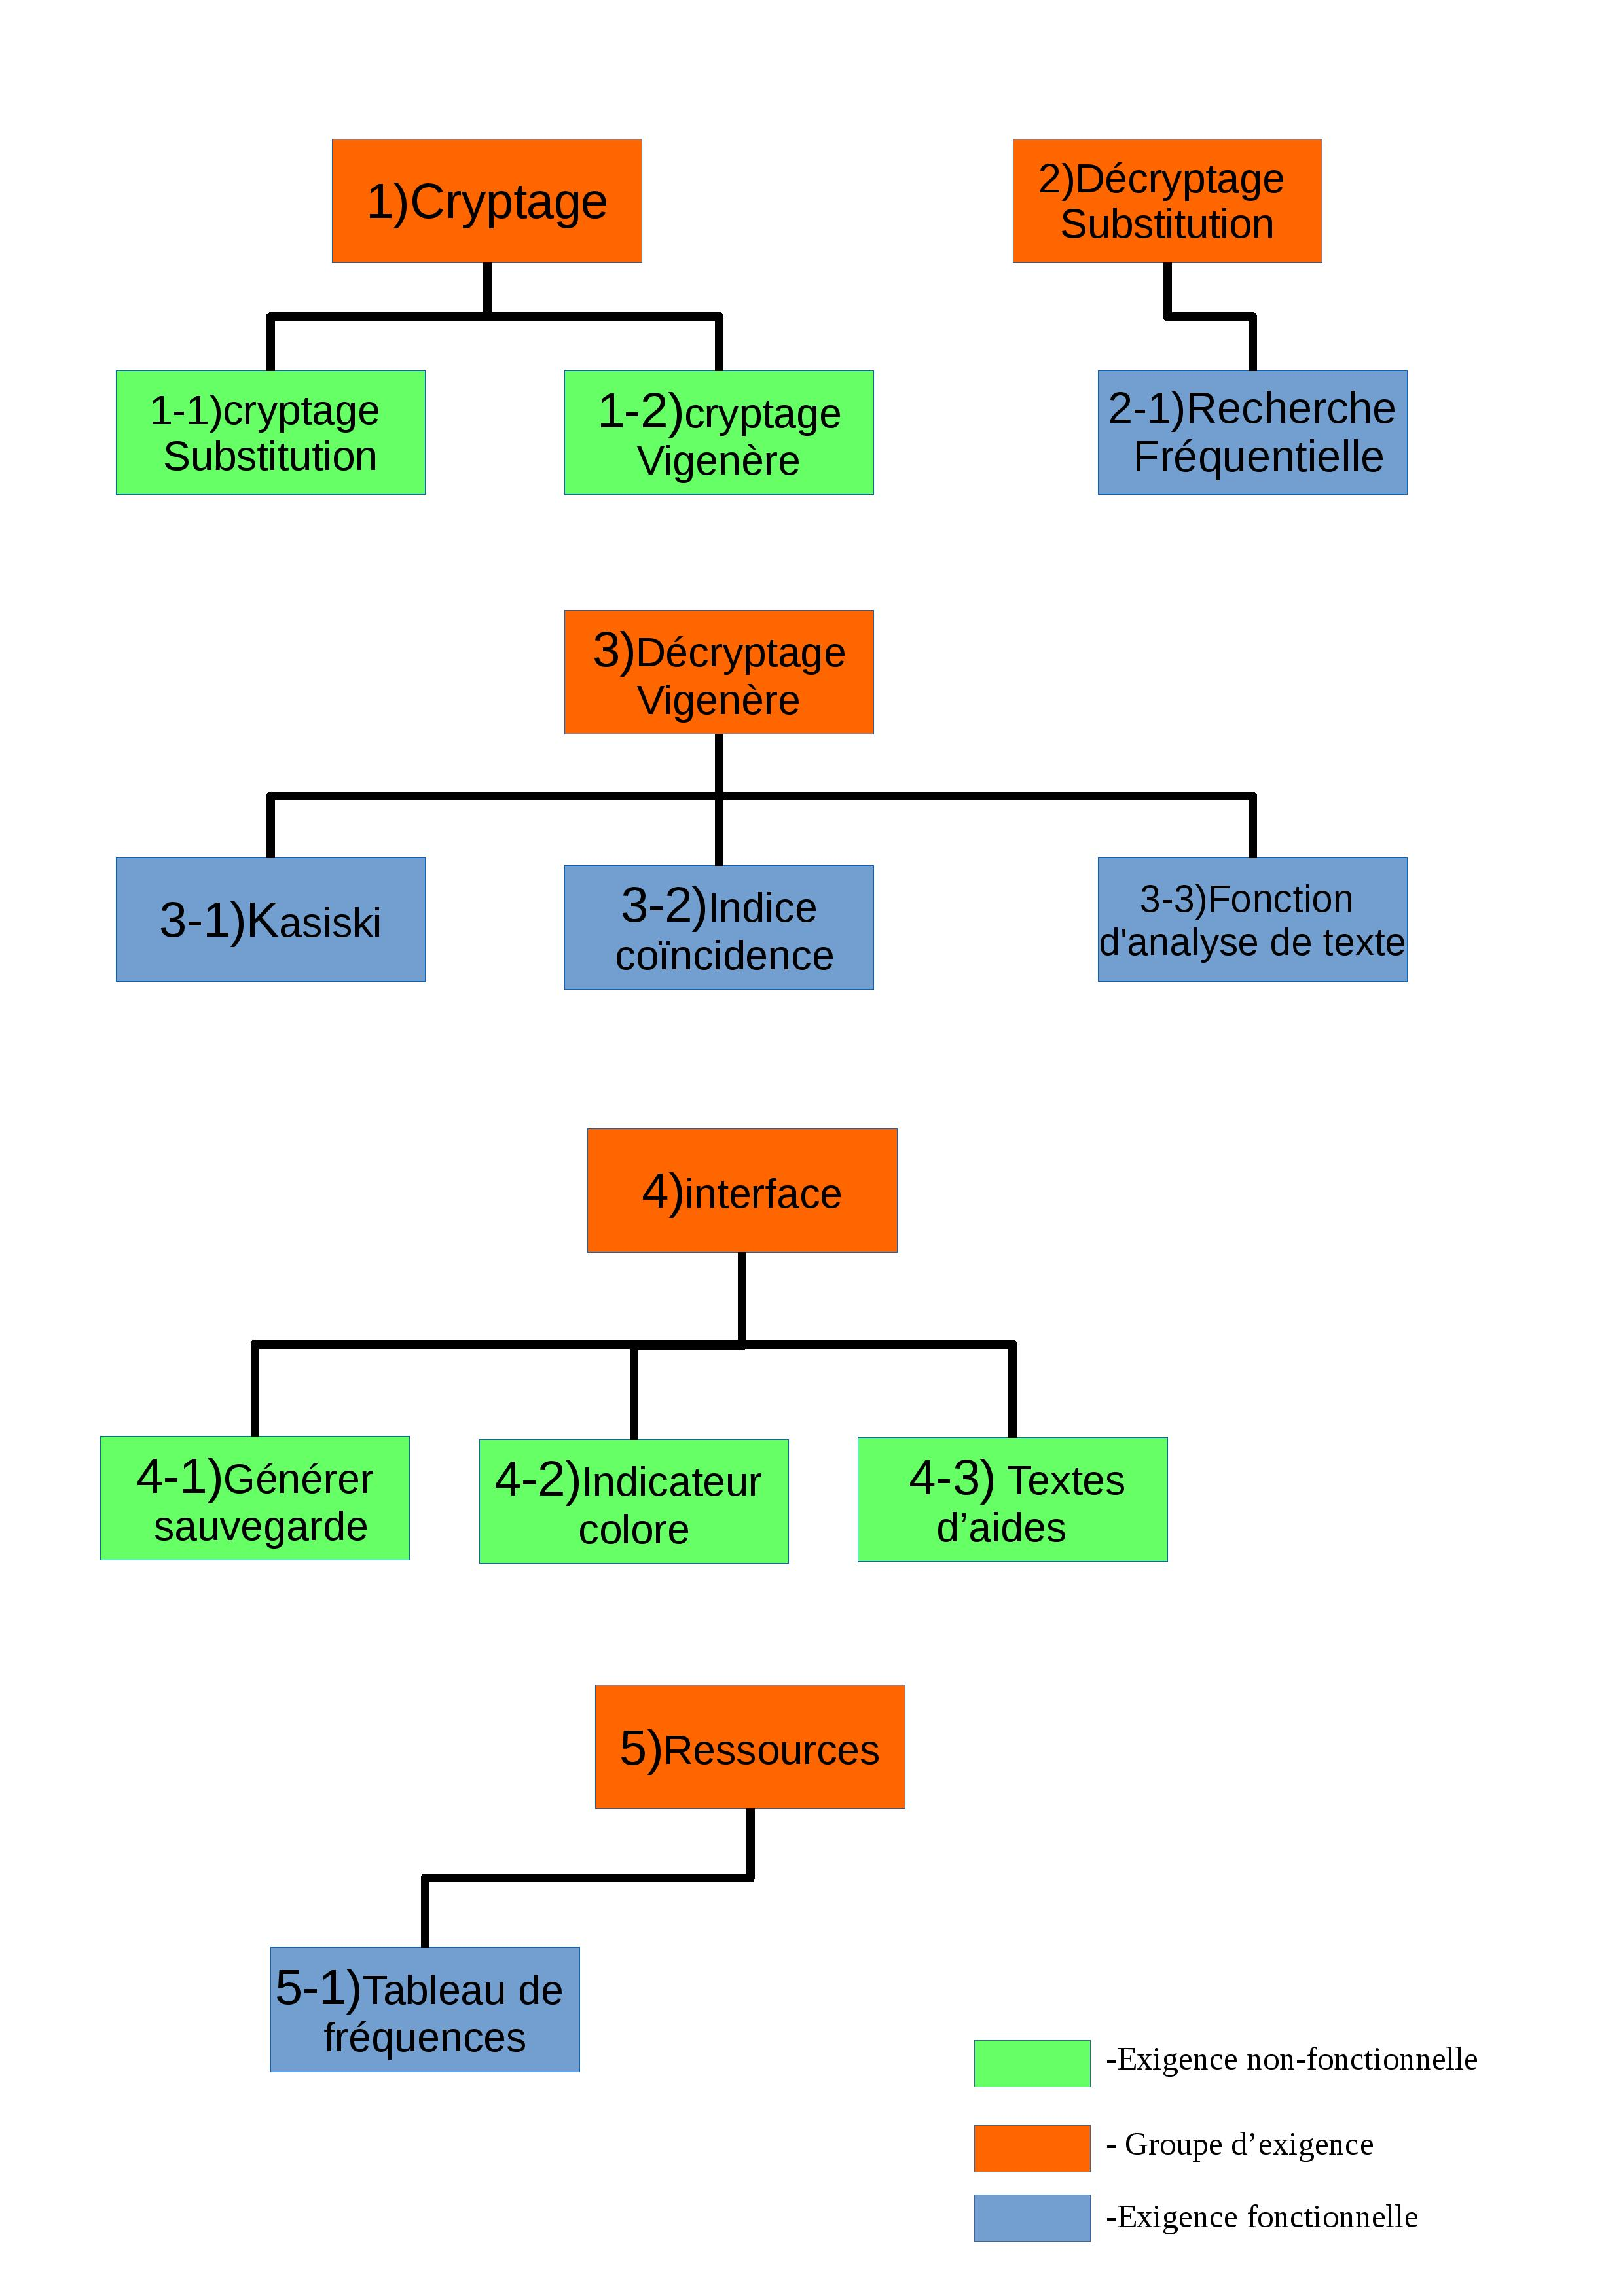
\includegraphics[scale = 0.2]{arbre.jpg} \pause 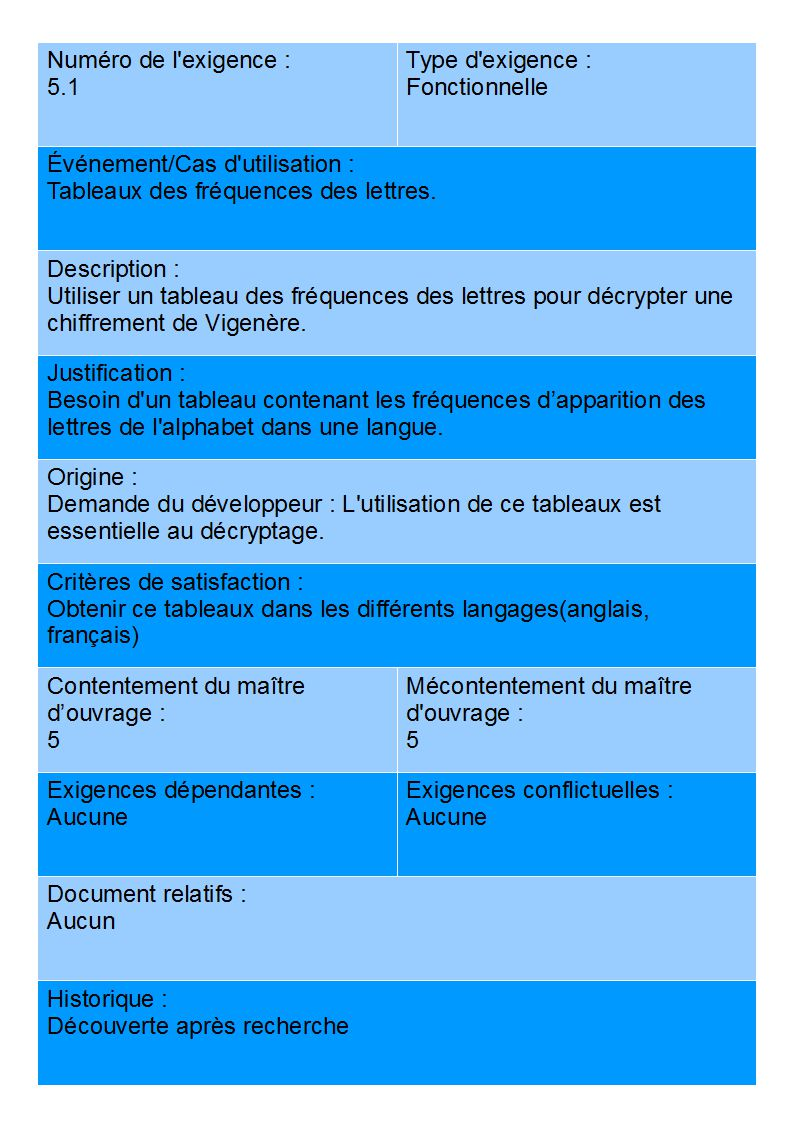
\includegraphics[scale = 0.5]{tab-freq.jpg} \pause 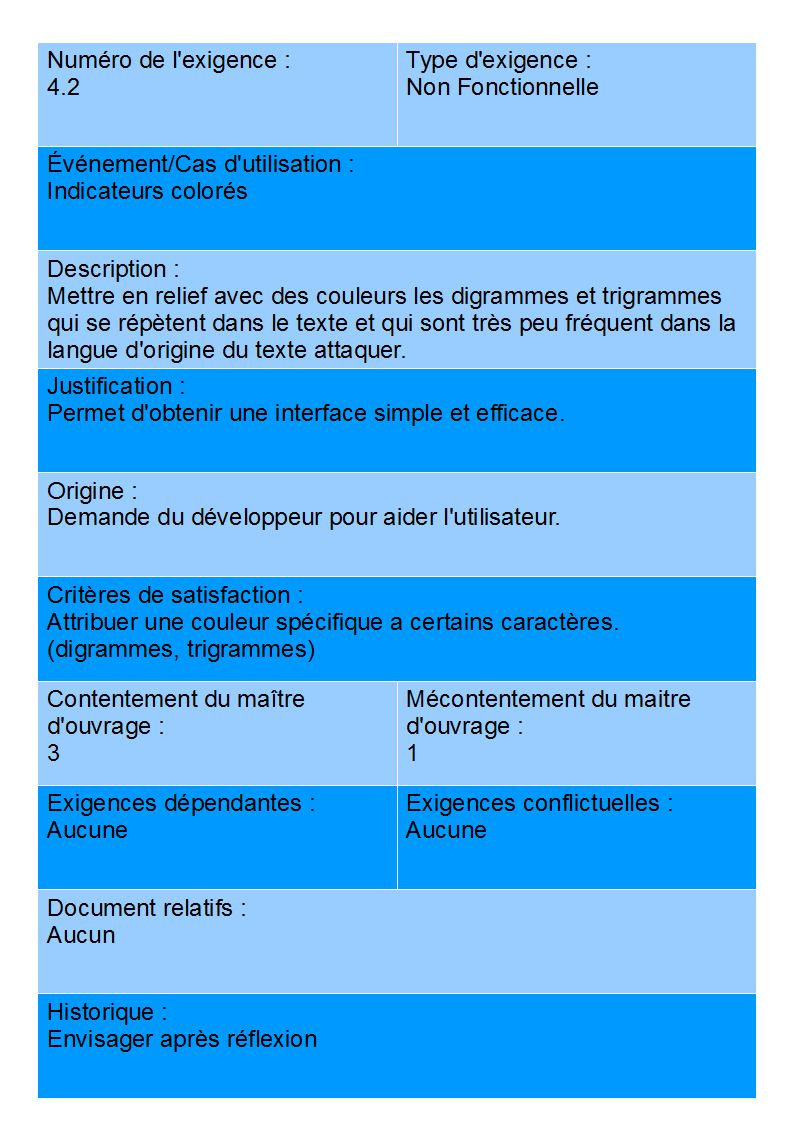
\includegraphics[scale = 0.5]{color.jpg}
\end{frame}
\begin{frame}
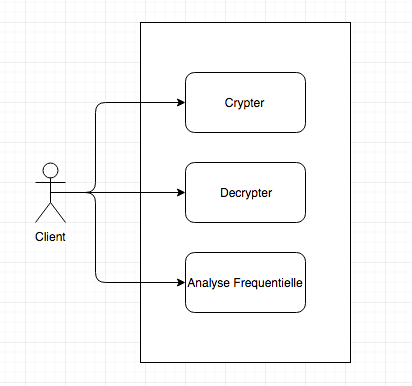
\includegraphics[scale = 0.5]{dia.png}
\end{frame}
%flo
\begin{frame}
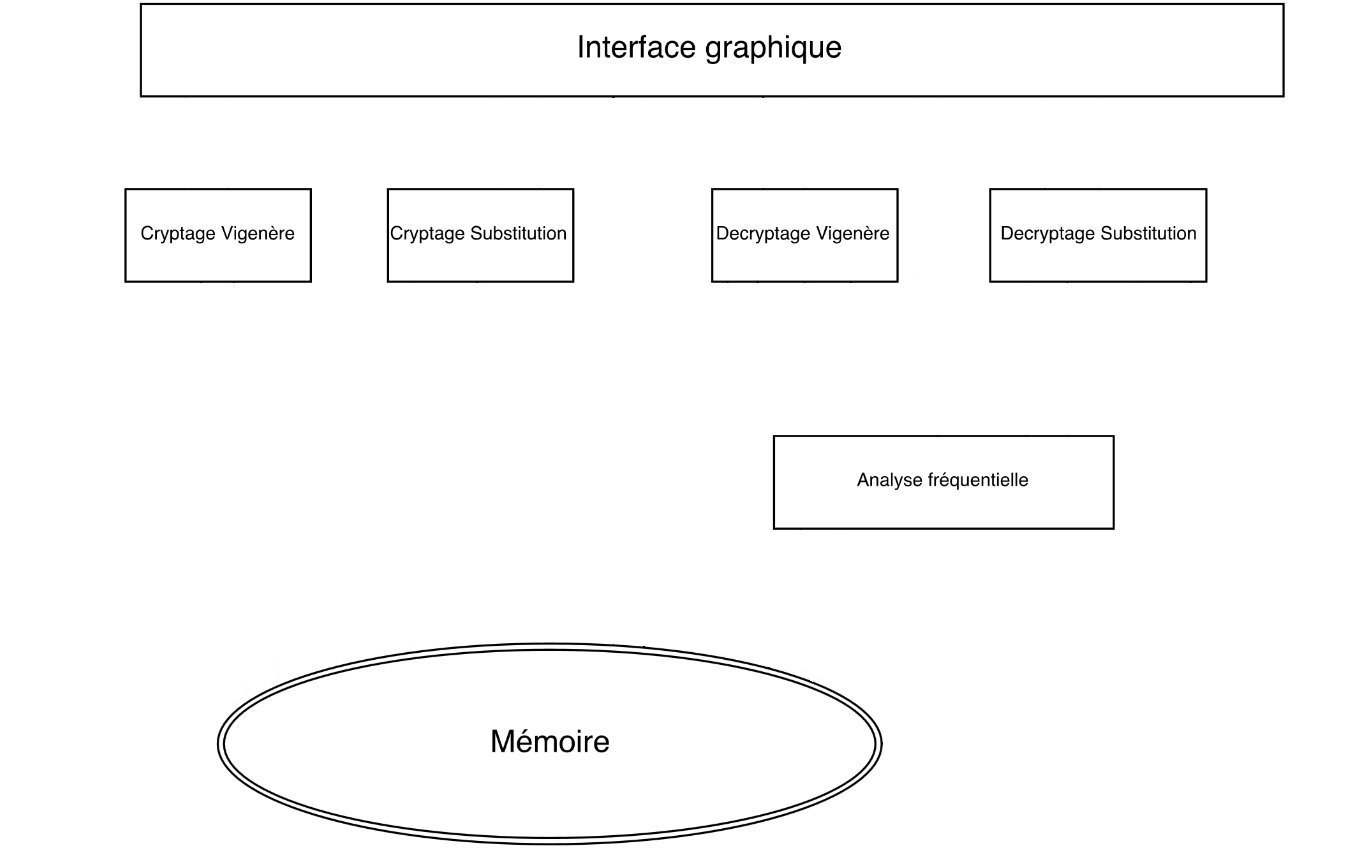
\includegraphics[scale = 0.22]{Org1.jpg}
\end{frame}
\begin{frame}
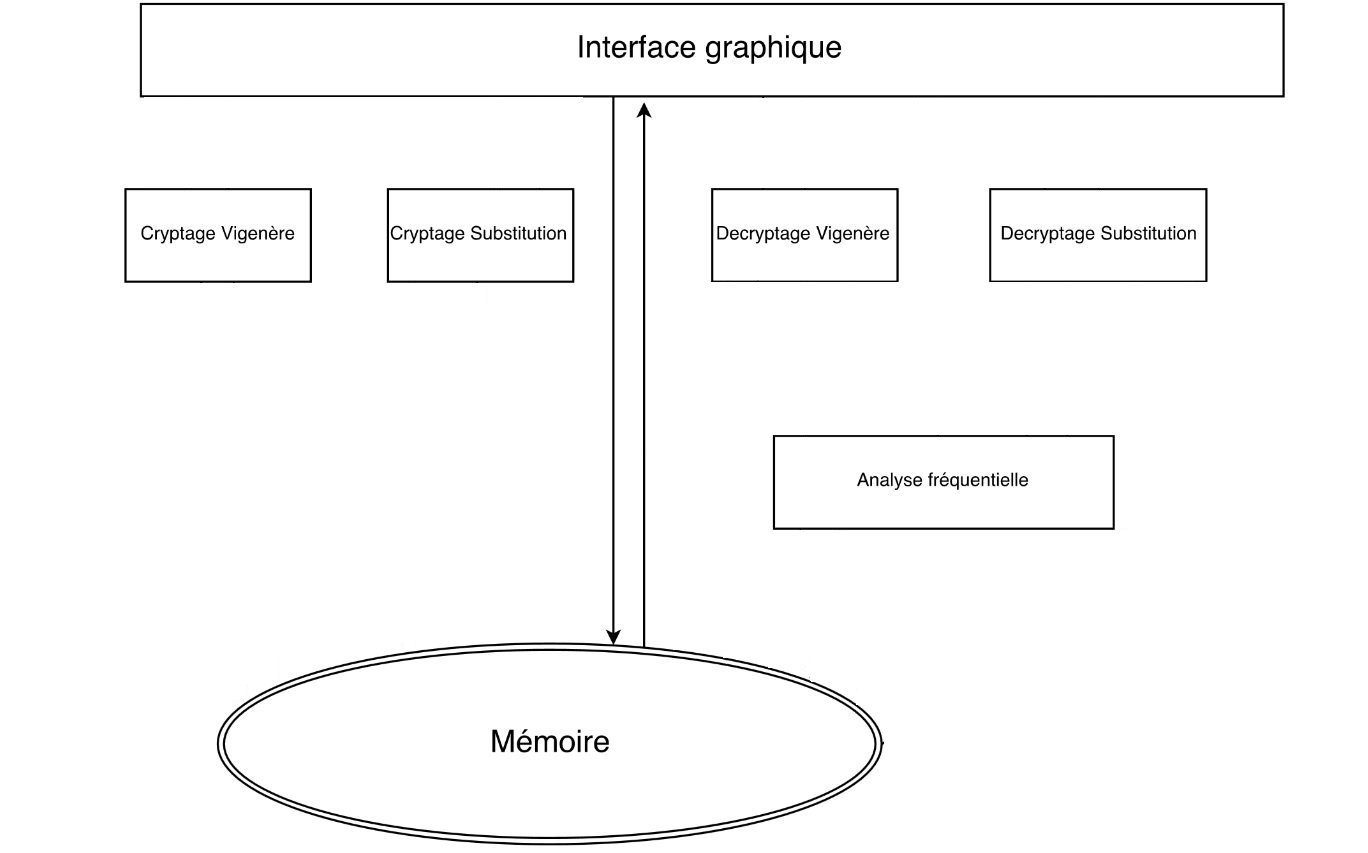
\includegraphics[scale = 0.22]{Org2.jpg}
\end{frame}
\begin{frame}
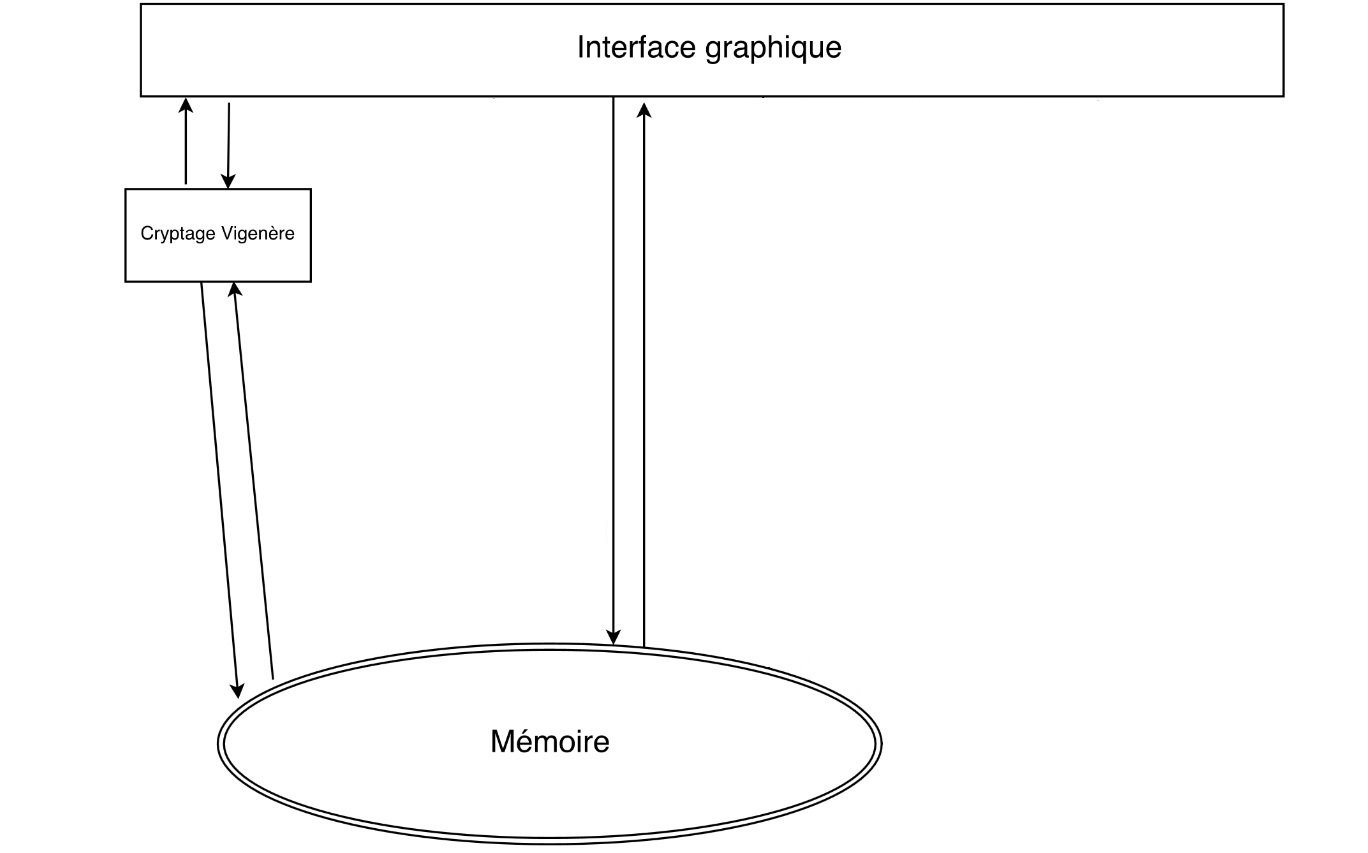
\includegraphics[scale = 0.22]{Org3.jpg}
\end{frame}
\begin{frame}
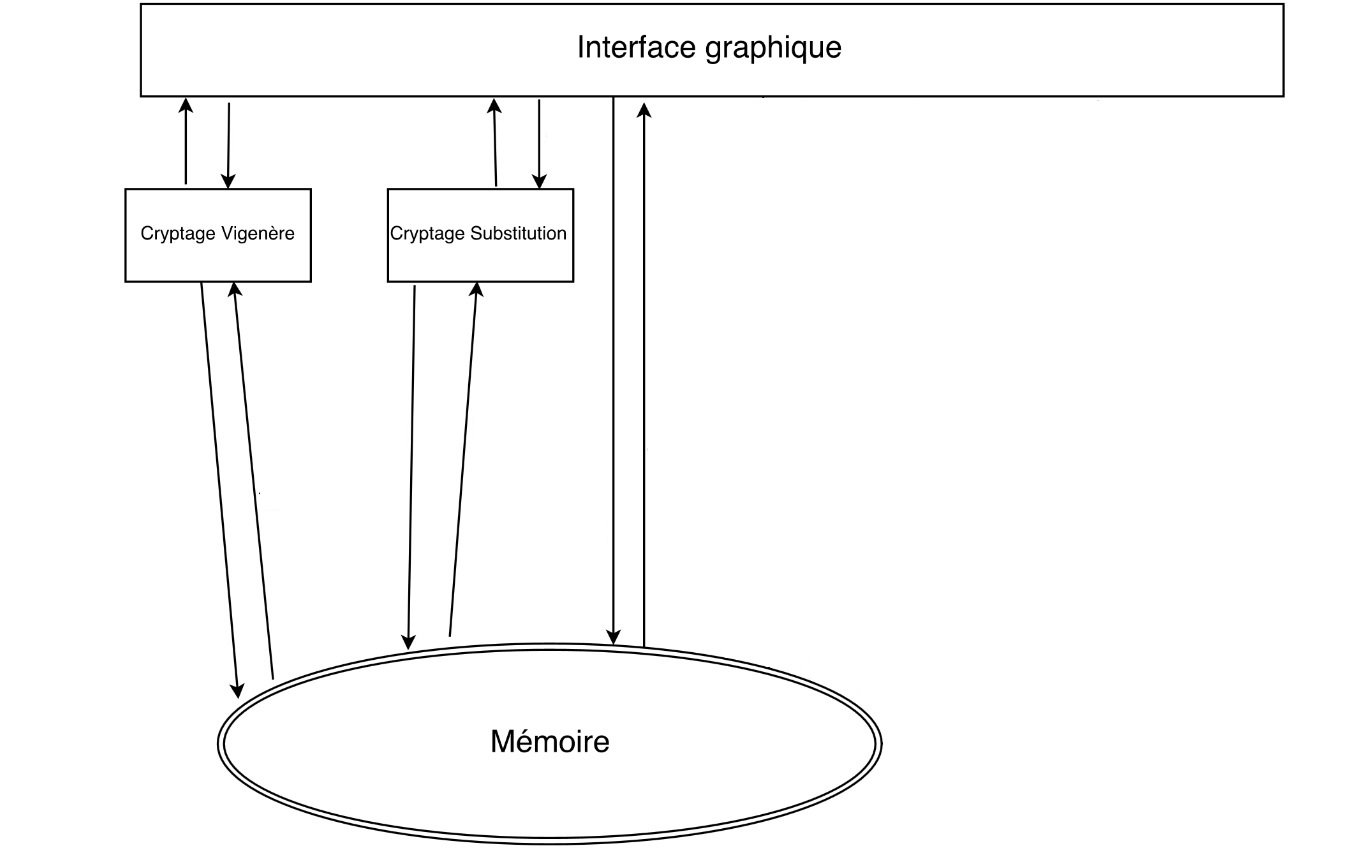
\includegraphics[scale = 0.22]{Org4.jpg}
\end{frame}
\begin{frame}
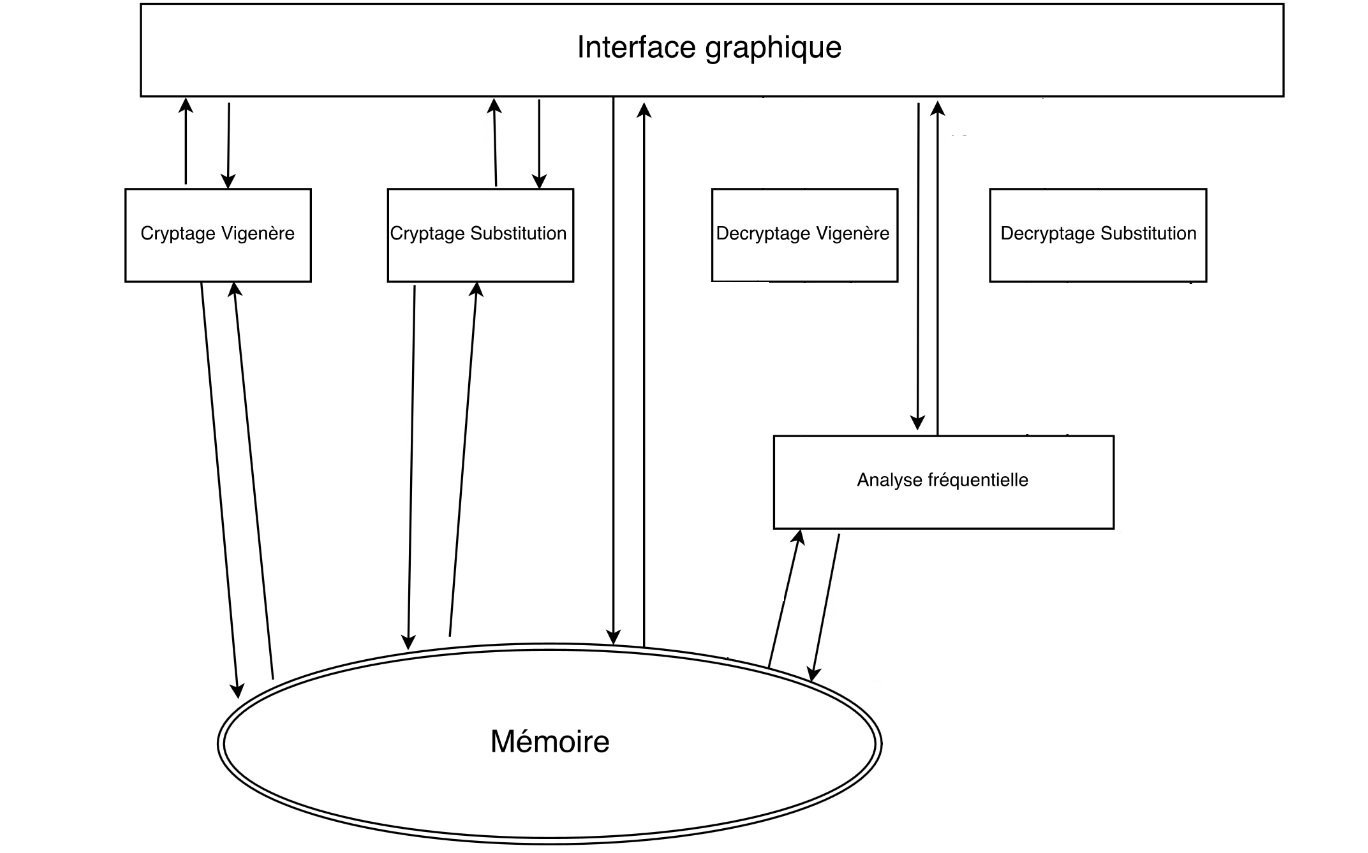
\includegraphics[scale = 0.22]{Org5.jpg}
\end{frame}
\begin{frame}
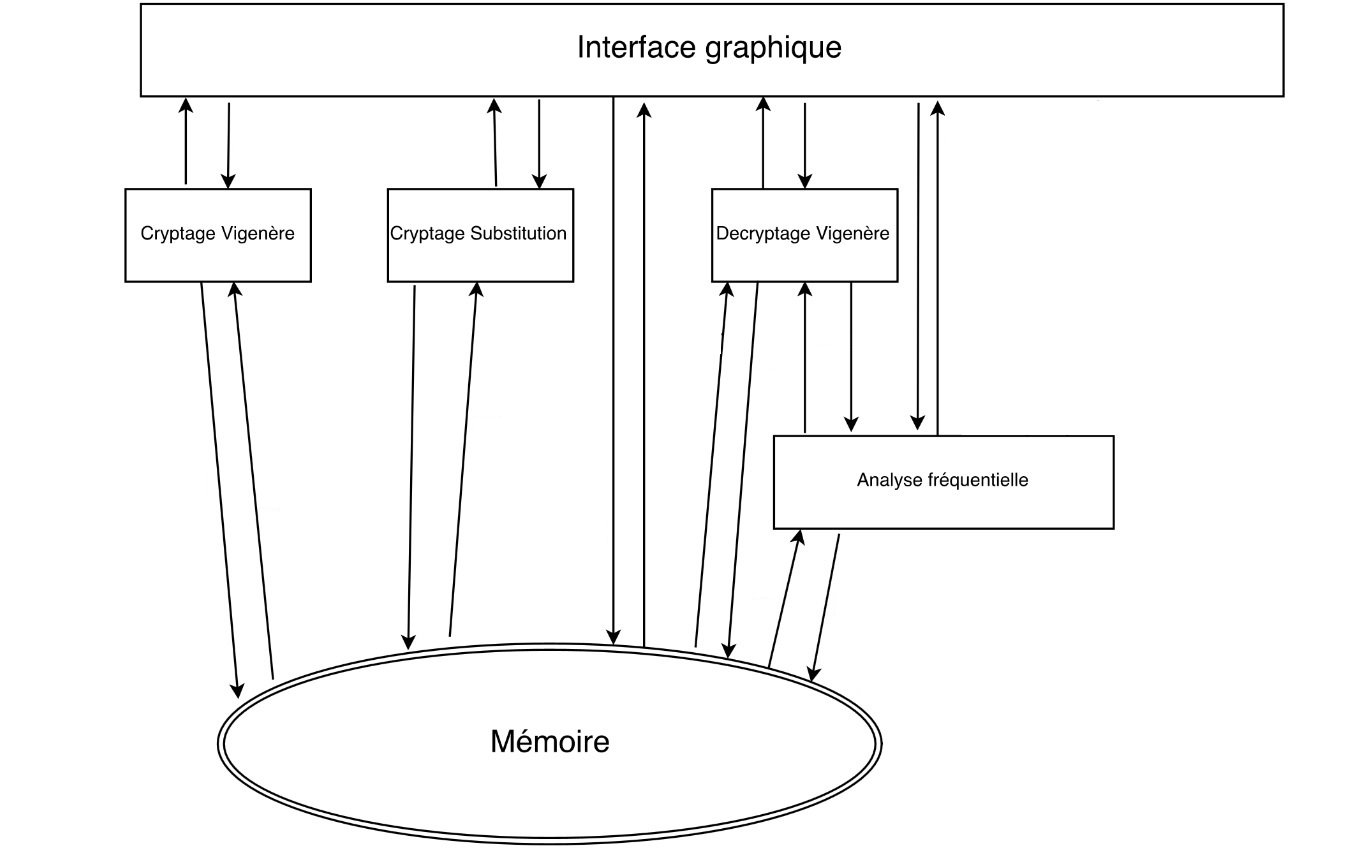
\includegraphics[scale = 0.22]{Org6.jpg}
\end{frame}
\begin{frame}
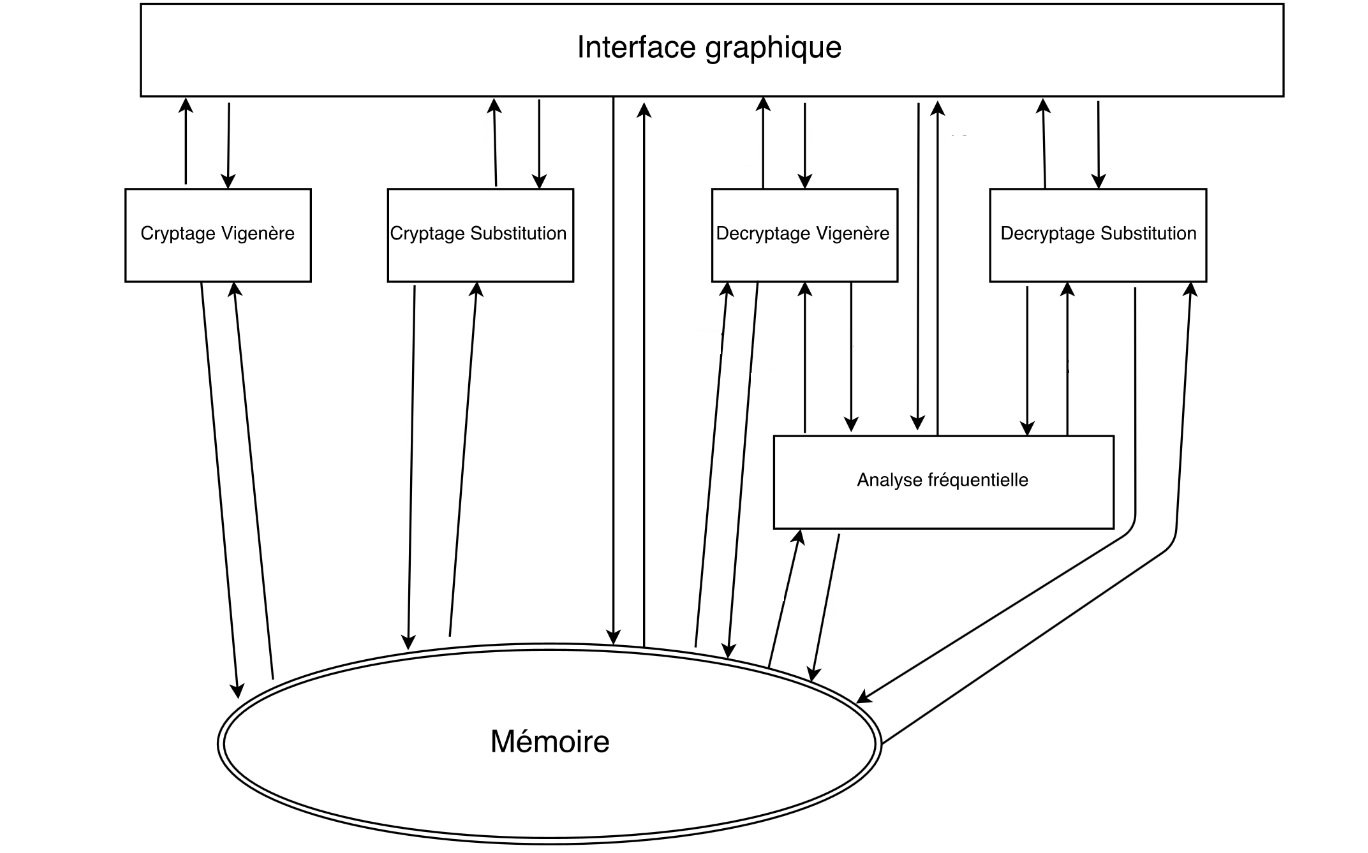
\includegraphics[scale = 0.22]{Org7.jpg}
\end{frame}
%abio
\begin{frame}
	\begin{block}{Hypothèse du coûts en nombre de ligne}
	\begin{center}
		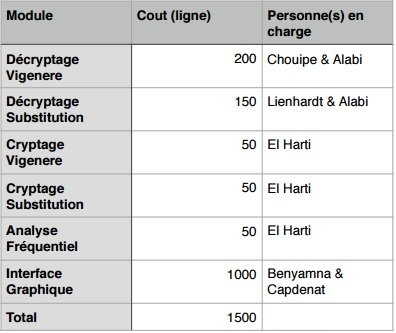
\includegraphics[scale =0.5]{Tableau_cout.jpg} \\ \pause
	\end{center}
	\end{block}
	\begin{block}{Choix du language}
	\begin{itemize}
		\item Language C \\ \pause
		\item Bibliothéque GTK 
	\end{itemize}
	\end{block}
\end{frame}
\begin{frame}
\begin{center}
\Huge {Conclusion}\pause
\end{center}
\begin{center}

\includegraphics[scale =0.5]{logo.png}
\end{center}
\end{frame}


\end{document}
